
% ----------------------------------------------------------------------
%                   LATEX TEMPLATE FOR PhD THESIS
% ----------------------------------------------------------------------

% based on Harish Bhanderi's PhD/MPhil template, then Uni Cambridge
% http://www-h.eng.cam.ac.uk/help/tpl/textprocessing/ThesisStyle/
% corrected and extended in 2007 by Jakob Suckale, then MPI-CBG PhD programme
% and made available through OpenWetWare.org - the free biology wiki


%: Style file for Latex
% Most style definitions are in the external file PhDthesisPSnPDF.
% In this template package, it can be found in ./Latex/Classes/
\documentclass[twoside,11pt]{Latex/Classes/PhDthesisPSnPDF}


%: Macro file for Latex
% Macros help you summarise frequently repeated Latex commands.
% Here, they are placed in an external file /Latex/Macros/MacroFile1.tex
% An macro that you may use frequently is the figuremacro (see introduction.tex)
% This file contains macros that can be called up from connected TeX files
% It helps to summarise repeated code, e.g. figure insertion (see below).

% insert a centered figure with caption and description
% parameters 1:filename, 2:title, 3:description and label
\newcommand{\figuremacro}[3]{
	\begin{figure}[htbp]
		\centering
		\includegraphics[width=1\textwidth]{#1}
		\caption[#2]{\textbf{#2} - #3}
		\label{#1}
	\end{figure}
}

% insert a centered figure with caption and description AND WIDTH
% parameters 1:filename, 2:title, 3:description and label, 4: textwidth
% textwidth 1 means as text, 0.5 means half the width of the text
\newcommand{\figuremacroW}[4]{
	\begin{figure}[htbp]
		\centering
		\includegraphics[width=#4\textwidth]{#1}
		\caption[#2]{\textbf{#2} - #3}
		\label{#1}
	\end{figure}
}

% inserts a figure with wrapped around text; only suitable for NARROW figs
% o is for outside on a double paged document; others: l, r, i(inside)
% text and figure will each be half of the document width
% note: long captions often crash with adjacent content; take care
% in general: above 2 macro produce more reliable layout
\newcommand{\figuremacroN}[3]{
	\begin{wrapfigure}{o}{0.5\textwidth}
		\centering
		\includegraphics[width=0.48\textwidth]{#1}
		\caption[#2]{{\small\textbf{#2} - #3}}
		\label{#1}
	\end{wrapfigure}
}

% predefined commands by Harish
\newcommand{\PdfPsText}[2]{
  \ifpdf
     #1
  \else
     #2
  \fi
}

\newcommand{\IncludeGraphicsH}[3]{
  \PdfPsText{\includegraphics[height=#2]{#1}}{\includegraphics[bb = #3, height=#2]{#1}}
}

\newcommand{\IncludeGraphicsW}[3]{
  \PdfPsText{\includegraphics[width=#2]{#1}}{\includegraphics[bb = #3, width=#2]{#1}}
}

\newcommand{\InsertFig}[3]{
  \begin{figure}[!htbp]
    \begin{center}
      \leavevmode
      #1
      \caption{#2}
      \label{#3}
    \end{center}
  \end{figure}
}


%%% Local Variables: 
%%% mode: latex
%%% TeX-master: "~/Documents/LaTeX/CUEDThesisPSnPDF/thesis"
%%% End: 

\usepackage[T1]{fontenc}
\usepackage{array}
\usepackage{pdfpages}
\usepackage{listings}

%\usepackage{graphics}
% or use the graphicx package for more complicated commands
%\usepackage{graphicx}

%: ----------------------------------------------------------------------
%:                  TITLE PAGE: name, degree,..
% ----------------------------------------------------------------------
\usepackage{graphicx}

      \textwidth 15cm
      \textheight 22cm
      \parindent 10pt
      \oddsidemargin 0.85cm
      \evensidemargin 0.37cm


\begin{document}

\thispagestyle{empty}

\begin{center}

Vrije Universiteit Amsterdam \hspace*{2cm} Universiteit van Amsterdam

\vspace{1mm}

\hspace*{-7.5cm}
\includegraphics[height=25mm]{00_frontmatter/figures/vu-griffioen.pdf}

\vspace*{-2cm}\hspace*{7.5cm}
\includegraphics[height=15mm]{00_frontmatter/figures/uva_logo.jpg}

\vspace{1cm}

{\Large Master Thesis}

\vspace*{1cm}

\rule{.9\linewidth}{.6pt}\\[0.4cm]
{\huge \bfseries Microservices communication: A case study comparing the communication of microservices with different communication tools\par}\vspace{0.4cm}
\rule{.9\linewidth}{.6pt}\\[1.5cm]

\vspace*{2mm}

{\Large
\begin{tabular}{l}
{\bf Author:} ~~Svava Hildur Bjarnadóttir ~~~~ (2640598)
\end{tabular}
}

\vspace*{2cm}

\begin{tabular}{ll}
{\it 1st supervisor:}   & ~~Rob van der Mei \\
{\it daily supervisor:} & ~~Lorena Salamanca ~~~~ (Picnic Technologies) \\
{\it 2nd reader:}       & ~~Patricia Lago
\end{tabular}

\vspace*{2.5cm}

\textit{A thesis submitted in fulfillment of the requirements for\\ the joint UvA-VU Master of Science degree in Computer Science}

\vspace*{1.8cm}

\today\\[4cm] % Date

\end{center}

\newpage


% ----------------------------------------------------------------------
       
% turn of those nasty overfull and underfull hboxes
\hbadness=10000
\hfuzz=50pt


%: --------------------------------------------------------------
%:                  FRONT MATTER: dedications, abstract,..
% --------------------------------------------------------------


%\language{english}


% sets line spacing
\renewcommand\baselinestretch{1.2}
\baselineskip=18pt plus1pt


%: ----------------------- generate cover page ------------------------

%\begin{center}
%\textit{``I am the master of my fate, I am the captain of my soul'' \\ from {\em Invictus}, by William Ernest Henley}
%\end{center}

%: ----------------------- cover page back side ------------------------
% Your research institution may require reviewer names, etc.
% This cover back side is required by Dresden Med Fac; uncomment if needed.

\newpage
%\vspace{10mm}
%1. First Reader: Name Surname
%
%\vspace{10mm}
%2. Daily Supervisor: Name Surname
%
%\vspace{10mm}
%3. Second Reader: Name Surname
%
%\vspace{10mm}
%4. Industrial Supervisor: Name Surname
%
%\vspace{20mm}
%Day of the defense:

%\vspace{20mm}
%\hspace{70mm}Signature from head of PhD committee:



%: ----------------------- abstract ------------------------

% Your institution may have specific regulations if you need an abstract and where it is to be placed in the document. The default here is just after title.


% Thesis Abstract -----------------------------------------------------


%\begin{abstractslong}    %uncommenting this line, gives a different abstract heading
\begin{abstracts}        %this creates the heading for the abstract page

Microservices have gained interest in the last years, often as an alternative to monolithic applications. Microservice architecture revolves around independent services communicating over network interfaces. For them to be a viable alternative to an application in which all components can communicate locally (as is the case in monoliths), it is important that the network communication is efficient and has good performance. REST (REpresentational State Transfer) over HTTP is the most commonly used method of communication in microservice systems, but in recent years GraphQL, gRPC and RSocket have all been introduced as alternatives to REST. This thesis aims to evaluate the suitability of these four technologies for microservices, both through a comparative analysis of their architectures and through performance experiments based on a case study for Picnic Technologies. The results of this evaluation indicate that RSocket and gRPC are well suited for inter-service communication, both showing good performance in multiple cases. Their differences lie mainly in their architecture, with gRPC being an RPC client-server framework built over HTTP/2 while RSocket is a binary protocol with symmetric interaction models intended for byte stream transport such as TCP. On the other hand, GraphQL and REST are both better suited for client-facing APIs. Performance-wise, GraphQL does especially well for complex use cases, while REST performs the worst overall out of the four. GraphQL's schema, graph-based approach and client defined queries make it a good choice for more complex microservice architectures.
\end{abstracts}
%\end{abstractlongs}


% ---------------------------------------------------------------------- 


% The original template provides and abstractseparate environment, if your institution requires them to be separate. I think it's easier to print the abstract from the complete thesis by restricting printing to the relevant page.
% \begin{abstractseparate}
%   
% Thesis Abstract -----------------------------------------------------


%\begin{abstractslong}    %uncommenting this line, gives a different abstract heading
\begin{abstracts}        %this creates the heading for the abstract page

Microservices have gained interest in the last years, often as an alternative to monolithic applications. Microservice architecture revolves around independent services communicating over network interfaces. For them to be a viable alternative to an application in which all components can communicate locally (as is the case in monoliths), it is important that the network communication is efficient and has good performance. REST (REpresentational State Transfer) over HTTP is the most commonly used method of communication in microservice systems, but in recent years GraphQL, gRPC and RSocket have all been introduced as alternatives to REST. This thesis aims to evaluate the suitability of these four technologies for microservices, both through a comparative analysis of their architectures and through performance experiments based on a case study for Picnic Technologies. The results of this evaluation indicate that RSocket and gRPC are well suited for inter-service communication, both showing good performance in multiple cases. Their differences lie mainly in their architecture, with gRPC being an RPC client-server framework built over HTTP/2 while RSocket is a binary protocol with symmetric interaction models intended for byte stream transport such as TCP. On the other hand, GraphQL and REST are both better suited for client-facing APIs. Performance-wise, GraphQL does especially well for complex use cases, while REST performs the worst overall out of the four. GraphQL's schema, graph-based approach and client defined queries make it a good choice for more complex microservice architectures.
\end{abstracts}
%\end{abstractlongs}


% ---------------------------------------------------------------------- 

% \end{abstractseparate}


%: ----------------------- tie in front matter ------------------------

\frontmatter
% Thesis Dedication ---------------------------------------------------

%\begin{dedication} %this creates the heading for the dedication page

%To ...

%\end{dedication}

% ----------------------------------------------------------------------
% Thesis Acknowledgements ------------------------------------------------


%\begin{acknowledgementslong} %uncommenting this line, gives a different acknowledgements heading
%\begin{acknowledgements}      %this creates the heading for the acknowlegments



%\end{acknowledgements}
%\end{acknowledgmentslong}

% ------------------------------------------------------------------------





%: ----------------------- contents ------------------------

\setcounter{secnumdepth}{3} % organisational level that receives a numbers
\setcounter{tocdepth}{3}    % print table of contents for level 3
\tableofcontents            % print the table of contents
% levels are: 0 - chapter, 1 - section, 2 - subsection, 3 - subsection


%: ----------------------- list of figures/tables ------------------------





%: ----------------------- glossary ------------------------

% Tie in external source file for definitions: /0_frontmatter/glossary.tex
% Glossary entries can also be defined in the main text. See glossary.tex
% 
%% this file is called up by thesis.tex
% content in this file will be fed into the main document

% Glossary entries are defined with the command \nomenclature{1}{2}
% 1 = Entry name, e.g. abbreviation; 2 = Explanation
% You can place all explanations in this separate file or declare them in the middle of the text. Either way they will be collected in the glossary.

% required to print nomenclature name to page header
%\markboth{\MakeUppercase{\nomname}}{\MakeUppercase{\nomname}}


% ----------------------- contents from here ------------------------


%\nomenclature{LSY}{ehbfuefebbfbjkjkebfjbfbfw} 
%\nomenclature{DEPC}{diethyl-pyro-carbonate; used to remove RNA-degrading enzymes (RNAases) from water and laboratory utensils}
%\nomenclature{DMSO}{dimethyl sulfoxide; organic solvent, readily passes through skin, cryoprotectant in cell culture}
%\nomenclature{EDTA}{Ethylene-diamine-tetraacetic acid; a chelating (two-pronged) molecule used to sequester most divalent (or trivalent) metal ions, such as calcium (Ca$^{2+}$) and magnesium (Mg$^{2+}$), copper (Cu$^{2+}$), or iron (Fe$^{2+}$ / Fe$^{3+}$)}



 

%\begin{multicols}{2} % \begin{multicols}{#columns}[header text][space]
%\begin{footnotesize} % scriptsize(7) < footnotesize(8) < small (9) < normal (10)

%\printnomenclature[1.5cm] % [] = distance between entry and description
%\label{nom} % target name for links to glossary

%\end{footnotesize}
%\end{multicols}



%: --------------------------------------------------------------
%:                  MAIN DOCUMENT SECTION
% --------------------------------------------------------------

% the main text starts here with the introduction, 1st chapter,...
\mainmatter

%\renewcommand{\chaptername}{} % uncomment to print only "1" not "Chapter 1"


%: ----------------------- subdocuments ------------------------

% Parts of the thesis are included below. Rename the files as required.
% But take care that the paths match. You can also change the order of appearance by moving the include commands.


% this file is called up by thesis.tex
% content in this file will be fed into the main document

%: ----------------------- introduction file header -----------------------
\chapter{Introduction}\label{sec:intro}


% ----------------------------------------------------------------------
%: ----------------------- introduction content ----------------------- 
% ----------------------------------------------------------------------



%: ----------------------- HELP: latex document organisation
% the commands below help you to subdivide and organise your thesis
%    \chapter{}       = level 1, top level
%    \section{}       = level 2
%    \subsection{}    = level 3
%    \subsubsection{} = level 4
% note that everything after the percentage sign is hidden from output



Microservice architecture has been one of the most popular software architecture patterns in the last years, likely bolstered by the fact that many of the largest tech companies in the world have adopted it (among those are Google \cite{googlemicroservices} and Netflix \cite{netflixmicroservices}). Like with any system that relies on distributed components working together to form a cohesive whole, how the microservices communicate is of utmost importance. Any communication over the network adds extra overhead that does not exist in a monolithic architecture, which means that the methods, protocols and frameworks used for the communication need to be highly performant and convenient to minimize this effect. In the 2018 survey \textit{Challenges of Microservices Architecture}, 2 out of every 5 developers noted that performance and response time were very important, both of which can be greatly affected by the communication technology employed \cite{ghofrani2018challenges}. Similarly, Viggiato et al. found that 48.3\% out of 122 respondents rated "Expensive remote calls" as important or very important challenges of microservices \cite{viggiato2018microservices}. In addition, Zimmerman identified 9 potential research topics related to microservices architecture, the fourth of which included the question "... is RESTful HTTP only one of several valid remote communication options in the microservices architect's toolbox, and, if so, what are the decision drivers when choosing an option?" \cite{zimmermann2016microservices}. Thus, the performance of microservices communication, the choice of technology for this purpose and the design of interfaces are all highly relevant and necessary topics of interest for microservices-focused literature.

\section{Problem statement and research questions}

This thesis was written as part of an internship at Picnic, Amsterdam. Picnic is a Dutch online grocery service which handles all the logistics of procuring groceries, taking orders, fulfilling them and delivering them to the customer's door, with most of the technology used being developed in-house (including the app used by customers for ordering groceries). Like many start-ups, Picnic started out with a monolithic architecture, but has in recent years been extracting functionality out of the monolith into smaller services in an attempt to transfer to a more modular, microservices-based ecosystem. Most of these microservices expose a RESTful HTTP-based API (see section \ref{sec:rest} for more details on REST) which is used for both between-services and client-server communications. As the Picnic ecosystem grows and more microservices are extracted, it is imperative to keep the system highly performant. It is in Picnic's best interest to investigate whether their current approach is really the best one, or whether performance gains could be made by switching to a new mode of communication. In addition, performance is not the only metric that matters when choosing a technology for remote communications. The chosen style, framework or protocol should ideally also complement the main architecture of the system as well as be convenient in use, development and maintenance. Thus, the following two research questions are posed in this thesis:

\begin{enumerate}
    \item Which communication patterns are suitable for microservices, in terms of architecture, interface design, features offered and efforts required to develop and maintain such a system?
    \item How much can the performance of communication between a web application and a system of microservices improve with these new techniques, compared to a RESTful API served over HTTP requests?
\end{enumerate}

The REST architectural style has been the main choice for developers building HTTP web services and APIs in the last 10 years. According to the 2020 developer survey by Rapid API, 62.5\% of respondents currently use REST in production \cite{rapid2020survey}. For microservices specifically, a similar trend can be observed. In the 2020 survey of IT experts \textit{State of Microservices} conducted by The Software House, 76.8\% of respondents said their microservices communicate with each other over HTTP \cite{stateofmicroservices}. However, other modes of communication have been slowly gaining traction in the last years. The three technologies chosen for comparison with REST over HTTP for this thesis were GraphQL, gRPC and RSocket.

GraphQL is a query language developed at Facebook and officially introduced in 2015 \cite{schrock2015blog}. It was not designed explicitly with microservices in mind, but it has seen growing interest as an alternative to REST for traditional HTTP-based APIs. According to the 2019 State of JS survey, 38.7\% of web developers have used GraphQL and would use it again, compared to 5\% in 2016. Additionally, 50.6\% of respondents had heard of it and would like to learn it \cite{stateofjs}. On the other hand, Google developed gRPC specifically for its internal microservices. According to the aforementioned Rapid API survey, 13.5\% of respondents use gRPC \cite{rapid2020survey}. gRPC is, as the name suggests, an RPC framework built over HTTP/2 which aims to offer better performance than traditional HTTP-based protocols, frameworks and styles \cite{aboutgrpc}. The last communication mode chosen for this thesis was RSocket. RSocket is a messaging protocol designed for byte stream transport and intended to support reactive microservices, originating from a Netflix project but currently supported by a number of industry leaders such as Facebook, Netifi and Pivotal \cite{netifi2017rsocket}. The reactive focus makes RSocket an interesting candidate for Picnic and any other company embracing the reactive philosophy.

\section{Methodology}
First, a literature study will be conducted to gain insight into the current landscape surrounding this problem area. This study will aim both to provide background information into the technologies and concepts covered in this thesis, as well as identify related literature and approaches.

The first research question will be answered with a comparative analysis of the four communication technologies, supported by the specifications of each as well as a literature review. First, each technologies' usage of transfer protocols will be discussed. Next, the contracting (or lack thereof) of service interfaces will be compared between the four technologies. In chapter \ref{sec:suitability}, each communication method's suitability for the microservices architecture will then be assessed based on the analysis in the preceding section. The second research question will be answered with a case study within Picnic and experimentation performed to assess the performance of each technology in a number of test cases mimicking real-world use cases, focused solely on fetching data (rather than updating or inserting it). The thesis will then conclude by combining the conclusions resulting from each research question and an attempt will be made to provide a recommendation for which communication technologies are suited to Picnic's use case.

% Thesis outline?


% this file is called up by thesis.tex
% content in this file will be fed into the main document

\chapter{Background} \label{sec:background}



% ----------------------- contents from here ------------------------
% 

In this chapter, the most relevant concepts, architectures and technologies will be covered, in order to provide detail for the proceeding chapters. First, microservices architecture will be explained and the most relevant definition of it identified. Next, REST, GraphQL, gRPC and RSocket will be covered. For each one, the motivation and basic principles will be elaborated on, as well as the basic concepts and functionality.

\section{Microservices Architecture}
In the last five years (since 2015), interest in microservices has exploded. When the keyword "microservices" is used to search on Google Scholar\footnote{https://scholar.google.com/}, 716 results are returned for the period 1980-2015. In contrast, the results from 2016-2020 are around 12,100. The general consensus for the origins of the term is a workshop of software architects in Venice, 2011 \cite{fowler2014microservices} \cite{zimmermann2016microservices}. However, a few earlier papers have used the term to describe similar concepts, although these definitions do not completely match up with the current generally accepted definitions. Interestingly, it can be seen that over time, the definitions have evolved into what they are now, rather than the term being redefined for a completely different purpose.
For reference, the current definitions describe microservices as small, narrow purpose, independently deployed web services which can be combined to form a larger system \cite{fowler2014microservices}.

The first mention of microservices as an architectural term within the computer science field can be found in a dissertation by Viswanathan from 1994 \cite{viswanathan1994publishing}. Viswanathan classifies wireless information services by their geographical scope, and defines microservices as services that cover an area in the range of a few miles. This definition is quite different from the current one, as "micro" refers not to the size of the service itself, but rather as a description of the physical domain it covers. In 2000, Andre and Segarra \cite{andre2000generic} used the term to describe subtasks of a larger service, which approaches the modern definition while still being distinct from it.
The 2002 student research paper "Vergleich Microsoft .NET mit Sun ONE" by Hockmann \cite{hockmann2002vergleich} (only available in German) contains a definition that is remarkably close to the current ones: microservices are defined as "discrete services which can be written in different languages and distributed on different platforms, and can be compiled together to form a complete web service". A similar definition can be found in the 2004 dissertation by Kim \cite{kim2004foundation}, where microservices are presented as "independently developable components that can be integrated together".

The unifying factors throughout the different definitions are that a microservice should be a single (or narrow) purpose independently deployable service which can be combined with other microservices to form a larger system. Different requirements are then added, e.g. that the microservice should interact via messages \cite{dragoni2017microservices} or be developed and maintained by a dedicated, cross-functional team which handles the entire stack and life cycle of the microservice (data management, code, deployment, maintenance) \cite{fowler2014microservices}. Some view microservices as simply the "right" way to do SOA (Software Oriented Architecture) \cite{zimmermann2016microservices} while others claim that it is a new style distinct from SOA, in part due to the wide range of architectures that have been labelled SOA, many of which differ significantly from microservices architecture \cite{fowler2014microservices}.

The definition used within Picnic fits best with the definition offered by Martin Fowler in his 2014 blog post simply titled "Microservices":
\begin{quote}
/textit{
    In short, the microservice architectural style is an approach to developing a single application as a suite of small services, each running in its own process and communicating with lightweight mechanisms, often an HTTP resource API. These services are built around business capabilities and independently deployable by fully automated deployment machinery. There is a bare minimum of centralized management of these services, which may be written in different programming languages and use different data storage technologies. \cite{fowler2014microservices}}
\end{quote}
This is the definition that will be used throughout this paper. Most importantly, no requirement is put on the mode of communication, neither internally (between microservices) nor externally (between the microservice ecosystem and its clients), aside from the requirement that the communication be "lightweight". 


\section{REST} \label{sec:rest}
The REST (REpresentational State Transfer) architectural style was developed by Roy Fielding and published in his 2000 doctoral dissertation \cite{fielding2000architectural}. At the time, the Web had been growing exponentially in size for a few years, beyond what Tim Berners-Lee and other early developers of the Web had designed it for. Fielding originally set out to describe the HTTP object model, but this effort quickly turned out to rather be an architectural style which, while designed with HTTP in mind, could be applied to any technology \cite{fielding2017reflections}. As Fielding phrased it:
\begin{quote}
\textit{
The goal has always been to maintain a consistent and correct model of how I intend the Web architecture to behave, so that it could be used to guide the protocol standards that define appropriate behavior, rather than to create an artificial model that would be limited to the constraints originally imagined when the work began. \cite{fielding2000architectural}}
\end{quote}
As an architectural style, REST has several constraints that dictate what the roles and features of, and relationships between, elements should be. However, the choice whether to enforce these constraints is up to the developer of the API. The six constraints of REST are:
\begin{enumerate}
    \item \textbf{Client-Server}: The system should be divided into client and server, with the client handling the user interface and the server handling the data storage. This constraint is driven by the principle of \textit{separation of concerns}.
    \item \textbf{Stateless}: Communication must be stateless, and any request cannot take advantage of stored context on the server.
    \item \textbf{Cache}: Data within a response should be labeled as cacheable to allow clients to reuse the data later, to minimize the amount of requests made.
    \item \textbf{Uniform interface}: Interfaces should be generalized, and implementations decoupled from the services they provide. The trade-off is that the information transferred is not in a form specific to the requesting application's needs.
    \item \textbf{Layered system}: The system should be divided into layers, where each component in a layer is only aware of the layer it is communicating with.
    \item \textbf{Code-On-Demand}: Client functionality can be extended by downloading and executing code in the form of applets or scripts, simplifying clients. This constraint is optional within REST.
\end{enumerate}

The main architectural element of REST is the \textit{resource}. A resource can represent a person, document, image, a collection of other resources or any other information that can be given a name. Resource identifiers are then used to refer to the resource, and this identifier is chosen by the author of the API. In Fielding's original dissertation, the only rule provided for how this should be done, is that the authority responsible for the assigned identifier should also ensure that the semantic validity of the identifier mapping should not change over time \cite{fielding2000architectural}. However, over the last two decades some general guidelines have been developed, which have been understood by many to be the "right" way to do REST. As an example, the book \textit{REST API Design Rulebook: Designing Consistent RESTful Web Service Interfaces} includes extensive rules such as "Underscores should not be used in URIs" and "A singular noun should be used for document names" \cite{masse2011rest}. When implemented over HTTP, the resource identifier is expressed as a URI, allowing for a tree-like representation of resources and sub-resources. Another key principle of REST is that methods to access and transform resources are the same for any kind of resource, e.g. if a REST API has a resource with the URI "/resource/{resourceId}" and a client invokes that endpoint with the HTTP GET method, the understanding is that the response will be a complete representation of the instance of that resource identified by the resource ID, no matter which resource it is \cite{fielding2017reflections}.

\section{GraphQL}
GraphQL is a graph query language designed by Facebook around 2012, and officially presented at a React.js conference in early 2015. It was developed during Facebook's move from HTML5-driven applications to native ones, and still to this day powers most interactions in the Android and iOS apps \cite{schrock2015blog}. The main motivation behind GraphQL was to serve as a communication protocol for Facebook's client applications, or as it is worded in the official specification for the language:
\begin{quote}
\textit{
    GraphQL is a query language designed to build client applications by providing an intuitive and flexible syntax and system for describing their data requirements and interactions \cite{graphql2018spec}.}
\end{quote}
The language and accompanying framework is now maintained by the GraphQL foundation, a neutral entity hosted by the Linux Foundation. It is still used by Facebook, and has also been adopted by prominent members of the software industry such as Atlassian, GitHub, Shopify, Pinterest, Twitter and Yelp \cite{graphqlusers}.

GraphQL is a query-based language for declarative data-fetching. GraphQL has five design principles:
\begin{enumerate}
    \item \textbf{Hierarchical}: Queries are structured hierarchically, and are shaped just like the data they return.
    \item \textbf{Product-centric}: GraphQL is driven by the requirements of the engineers of the front-end clients.
    \item \textbf{Strong-typing}: Each server defines a type system specific to its own structure. This type system is used to validate queries and make guarantees about the shape and format of the response.
    \item \textbf{Client-specified queries}: Each server, through a schema, publishes the different functions available to clients. Clients specify how they want to use these functions and which fields and objects they want returned. This ensures that clients never receive data that they didn't specifically ask for.
    \item \textbf{Introspective}: The type system of each server must be queryable by the GraphQL language itself, which in essence allows clients to request the schema itself. This helps clients know exactly which fields and types are available to them, and can even allow them to validate their queries before sending them to the server.
\end{enumerate}

\begin{lstlisting}[caption={An example GraphQL schema}, captionpos=b,label={lst:schema}]
    type Query {
      getUser(id: Int): User
      getUsers: [User]
    }
    
    type User {
      id: Int
      name: String
      friends: [User]
    }
\end{lstlisting}
A minimal example of a GraphQL schema can be seen in Listing \ref{lst:schema}. The schema defines a single type, a User with two primitively typed fields, and one which refers to a collection of other User typed objects. It is then up to the server's specific implementation how this is stored in a database and retrieved before being returned to the client. The schema also defines a single query type, which defines the queries available for clients to use. In this case, two queries are available. The first accepts a single \texttt{id} parameter and returns the user identified by that ID. The second accepts no parameters and returns a collection of (presumably) all the users stored by the server. Listing \ref{lst:query} shows an example usage of the first query. Noticeably, the query actually allows the client to fetch much more than could be expected: since each friend is a User type, the client can recursively query the friends of each of those friends.

\begin{lstlisting}[caption={An example GraphQL query}, captionpos=b,label={lst:query}]
{
  getUser(id:12345) {
    name
    friends {
      name
      friends {
        name
      }
    }
  }
\end{lstlisting}

\section{RSocket}
RSocket is a reactive message-based OSI layer 7 protocol announced in September 2018 at the SpringOne Platform conference in Washington DC. It is developed and supported by Netifi (founded by members of the team that created the RSocket project at Netflix), Facebook and Pivotal \cite{netifi2017rsocket} and is now maintained by the Reactive Foundation, hosted by the Linux foundation \cite{melanson2019rsockethome}. The foundation's members include large tech companies such as Facebook, VMWare and AliBaba \cite{reactivemembers}. 

The development of RSocket was driven largely by the need for a communication protocol that embraces the principles of the Reactive Manifesto \cite{rsocketmotivations}.  The following list summarizes the motivations and key design principles of RSocket:

\textbf{Message-driven}: All communication is modeled as non-blocking streams of messages over a single network connection.

\textbf{Interaction models}: Beyond the typical behavior of client-server architectures, RSocket offers the following four interaction models:
    \begin{itemize}
        \item \textit{fire-and-forget}: The client sends a one-off message to the server without expecting or receiving a response.
        \item \textit{request-response}: The client sends a request and receives a single message.
        \item \textit{request-stream}: The client sends a request and receives a stream of messages.
        \item The client and server set up a channel where the client can send multiple messages, expecting one or more response messages per message sent.
    \end{itemize}

\textbf{Behavior}: RSocket supports bi-directional requests, allowing both client and server to act as requester and responder. In addition, any stream can be cancelled by the requester allowing the responder to terminate early.

\textbf{Resumability}: Sessions can easily be resumed after network failures or disruptions with a simple handshake.

\textbf{Flow control}: Two forms of flow control are implemented. Firstly, the requester can dictate exactly how many messages it wants to receive at a time to prevent it from being overloaded. Secondly, a responder can issue a lease to the requester, which means that the requester knows that the server is not at full capacity, and can still receive requests.

\textbf{Polyglot support}: The RSocket protocol provides a contract for the behavior between the client and server. Thus, it does not matter which languages each is written in, as long as they adhere to the contract.

\textbf{Transport Layer Flexibility}: RSocket is not tied to TCP and is expected to work over any protocol with similar features (WebSockets, Aeron, QUIC).

\textbf{Efficiency and Performance}: RSocket aims to improve performance by (among other things) avoiding handshakes as much as possible, using binary encoding and allocating less memory.

\section{gRPC}
gRPC is a remote procedure call (RPC) framework developed at Google in 2015 \cite{marculescu2015introducing}. Besides powering Google's microservices infrastructure, gRPC is currently used by companies such as Cisco, Netflix and Square \cite{aboutgrpc}. gRPC was developed as the open-source next version of Stubby, a non-standardized RPC infrastructure used for Google's internal microservices \cite{ryan2015motivation}. gRPC was designed to be a open-source, free framework which promotes the microservices design philosophy of message exchange.

gRPC, like other RPC systems, is based around the idea of allowing clients to invoke remote server methods just as they would local methods. The server implements methods described by an interface and the client uses a \textit{stub} which offers the methods described by the interface. gRPC uses \textit{protocol buffers} to serialize structured data, which offers advantages over JSON such as field types, field IDs and rules (repeated, optional and required fields) \footnote{It is important to note that gRPC does not require using protocol buffers, and protocol buffers can be used with any transfer protocol. However, they are both developed by Google and gRPC uses protocol buffers by default. Most documentation recommends using protocol buffers for serialization and interface contracting. Thus this thesis will in most cases assume that protocol buffers are used with gRPC}. 
gRPC is built on top of HTTP/2 and uses a traditional client/server interaction model, wherein the client can only request data from the server through the methods defined by the protocol buffer interface. gRPC offers both a blocking and non-blocking API, allowing clients to either synchronously or asynchronously request data from the server. gRPC also offers extensive features such as flow control, cancellations, lameducking and streaming \cite{ryan2015motivation}. Beyond the simple request-response functionality, the three modes of streaming offered in gRPC are the following \cite{grpccore}:
\begin{itemize}
    \item \textit{Server streaming}: The client sends a single request and receives a stream of messages in response.
    \item \textit{Client streaming}: The client sends a stream of messages and receives a single message in response.
    \item \textit{Bidirectional streaming}: The client initiates a call and sends a stream of messages to the server, which responds with a stream of messages. The streams are independent and it is up to each to decide how many messages to stream in response to each message received.
\end{itemize}



% ---------------------------------------------------------------------------
% ----------------------- end of thesis sub-document ------------------------
% ---------------------------------------------------------------------------

\chapter{Related work}\label{sec:related}
In this chapter, literature and papers related to this paper's subject will be reviewed. First, literature relating to microservices, their performance and choice of communication technology will be documented. Next, papers that aim to compare any of the four communication technologies (REST, GraphQL, RSocket and gRPC) or related technologies will be covered, first in general and then specifically in the context of microservices.

\section{Microservices performance}
As mentioned earlier, the interest in microservices has exploded in the last few years. In a Google Scholar search initiated at the time of writing this paper, around 17,500 results are returned when searching for papers containing the word \textit{microservices} in the title. However, few of them are focused explicitly on both communication and performance. As mentioned in chapter \ref{sec:intro}, the three papers by Ghofrani, Viggiato and Zimmerman (respectively) all serve as overviews of the state of practice and research into microservices \cite{ghofrani2018challenges} \cite{viggiato2018microservices} \cite{zimmermann2016microservices}. Ghofrani and Viggiato both found that performance of remote communications in microservices were rated as important challenges by professionals, while Zimmermann questioned the status of RESTful HTTP as the de facto communication technology of microservices. In Soldani's 2018 review of grey literature identifying pains and gains of microservices, API versioning, communication heterogeneity and service contracts are identified as pains, which are all highly relevant to the choice of communication technology for microservices \cite{soldani2018pains}. Finally, in the 2017 article \textit{Processes, Motivations, and Issues for Migrating to Microservices Architectures} by Taibi, Lenarduzzi and Pahl \cite{taibi2018architectural}, communication among services is named as a drawback to the microservices architecture as it adds complexity to the implementation as well as causing possible latency issues, both of which could potentially be addressed by using a communication technology better suited to the architecture.

A number of studies were found that analyzed the performance of microservices, but these were more focused on either comparing microservices to other architectures, or investigating the effects of the infrastructure on the performance. Ueda, Nakaike and Ohara fall into the first camp. They analyzed the performance of microservice-based systems in their 2016 report \textit{Workload Characterization for Microservices} \cite{ueda2016workload}. Their goal was to compare microservices to monolithic applications, however they did show that the microservice-based application spent more time in communication libraries than the monolithic one, indicating that improving the communication performance of microservices could minimize the gap in performance between microservices-based architectures and monolithic ones. Similarly, Gan and Delimitrou showed that in a microservice-based system, communication is a more significant bottleneck than computation when compared with the same application written as a monolith \cite{gan2018architectural}. On the other hand, Amaral et al. \cite{amaral2015performance} and Kratzke \cite{kratzke2017microservices} each performed research on the performance of microservices, but both focused on the impact of containers (e.g. Docker) and the underlying infrastructure used to deploy the services, rather than the design or architecture of the microservices themselves.

\section{Communication technologies in web services}
A number of papers have been published which compared GraphQL to REST APIs in terms of either architecture or performance, but not specifically for microservices. Eizinger's 2017 master thesis compared REST and GraphQL in terms of API design, finding that using GraphQL shifts responsibilities from the client to the server \cite{eizinger2017api}. Vogel et al. conducted experiments on the same server, one before migrating fro mREST to GraphQL and one after and found that for a single request the performance was similar. However, for cases where multiple resources were required, GraphQL was faster due to a reduction in the number of requests needed \cite{vogel2017experiences}. Similarly, Vázquez-Ingelmo et al. migrated a system from REST to GraphQL and observed a decrease in average response time due to a reduction of request volume \cite{vazquez2017improving}. Finally, Cederlund performed experiments on the same system developed with either REST or GraphQL, and showed similar results as Vogel et al. with a similar performance in single-resource test cases but increased performance by GraphQL in multiple-resource test cases \cite{cederlund2016performance}.

However, as far as the author knows, few research-based literature has been published comparing either REST or GraphQL to gRPC and RSocket. Chamas, Cordeiro and Eler analyzed the energy cost differences of REST, SOAP, Socket and gRPC, however they did not consider the performance (e.g. speed) of the technologies \cite{chamas2017comparing}. Multiple papers have been written that seek to compare and contrast REST with RPC frameworks in general, however these are less relevant since even though gRPC is an RPC-based framework, the papers focus mostly on SOAP or other synchronous RPC approaches (while gRPC can be both synchronous and asynchronous) \cite{mironela2009importance,feng2009rest,aboutgrpc,vinoski2008rpc,kennedy2009framework}. Similarly, Socket communications have been compared with REST \cite{choi2012performance,cho2014replacing}, however RSocket offers functionalities beyond plain socket communications which these comparisons do not take into account.

\section{Communication technologies in microservices}
For analysis of architecture or performance of communications specifically in microservices, a limited number of papers exist. Hong, Yang and Kim conducted a performance analysis of RESTful APIs versus RabbitMQ for microservices, finding that RabbitMQ (a message broker and queueing server \cite{rostanski2014evaluation}) performed better than REST, with more stability in situations of load \cite{hong2018performance}. However, this thesis focuses more on comparing frameworks and protocols that are centered around direct message transport rather than queueing systems. For this reason, RabbitMQ was not included in the evaluation. 

Nguyen performed experiments to compare the performance of three RPC-based frameworks in microservices architecture in her 2016 thesis, concluding that even though gRPC did not have the best performance in all cases, it is a good choice for a microservices architecture based on other advantages, such as extensive documentation, active development and a "modern style" \cite{nguyen2016benchmarking}.

The paper most directly related to this thesis (and the original inspiration for it) is the 2017 master's thesis \textit{Efficient Communication With Microservices} by Johansson \cite{johansson2017efficient}. Johansson compared the performance of REST over HTTP with JSON with GraphQL and found that GraphQL was slower in all cases. However, there were issues with his methodology and experiment design. None of his test cases showcased the most prominent benefit of GraphQL: that fewer requests are needed to fetch the same data. Thus, his conclusion that GraphQL has a worse performance than REST is incomplete. In addition, he included a small section on gRPC and Apache Thrift, but did not provide arguments supporting his decision to not include those in the performance comparison.

\chapter{Architecture comparison}\label{sec:comparison}
In this chapter, a comparative analysis of the four technologies will be conducted. First, the choice and usage of transfer protocols for each will be investigated, with a focus on improvements over HTTP/1.1. Then, the approaches each technology uses for interface design and contracting will be compared.

\section{Transfer protocols}\label{sec:transfer}
For microservices, communication is usually done via HTTP \cite{zimmermann2016microservices}, and before the release of HTT/2 in 2015, that was via HTTP/1.1. From 1999 until 2014, the HTTP/1.1 standard remained unchanged \cite{rfc2616}. One of the prominent issues with HTTP/1.1 is the fact that, for each transaction, a new connection must be established which increases overall latency when performing multiple requests \cite{spero1994analysis}. 

Since REST was designed with HTTP in mind, it is rarely used with anything else (although that is possible). That means that RESTful APIs usually suffer from this performance issue of HTTP/1.1. Furthermore, since a URI should only ever refer to a single resource within REST\cite{masse2011rest}, when a client needs to fetch multiple resources, multiple requests need to be issued and in turn, multiple connections need to be established.

GraphQL, while similarly platform independent yet rarely implemented over anything but HTTP/1.1, attempts to mitigate this issue by reducing the amount of requests needed to be made. By allowing clients to refer to any related resources in their queries, the overall request volume needed to fetch data can be decreased, improving performance \cite{schrock2015blog}. In the 2017 study on the performance differences between REST and GraphQL mentioned in chapter \ref{sec:related}, Vázquez-Ingelmo et al. found that the average response time of loading a specific dashboard decreased by 2 seconds, largely due to the fact that in REST, the action required 17 requests while with GraphQL, one was sufficient \cite{vazquez2017improving}.

gRPC however, is designed for and bound to HTTP/2. HTTP/2 is a new version of HTTP which adds multiplexing, allowing clients to send and receive more than one request/response message over the same connection \cite{rfc7540}. This allows gRPC clients to avoid the latency induced by having to re-establish a connection for each request, improving the overall performance. In addition, gRPC has no constraints or guidelines on the semantics of methods defined, meaning that if desired, developers can create methods that fetch all the data needed in a single request. Finally, HTTP/2 includes the feature of header compression, whereas in HTTP/1.1 headers are uncompressed and sent in plain text. This enables HTTP/2 payloads to be overall smaller, saving on bandwidth \cite{rfc7540}.

Finally, RSocket can bypass the issues of HTTP entirely. RSocket is a protocol defined at the same level as HTTP and works over binary, duplex protocols such as TCP. RSocket thus can also enjoy the benefit of multiplexing. Further, unlike all versions of HTTP currently in use, RSocket allows both the client and the server to act as sender and receiver. In a system that relies on e.g. push notifications, this can improve performance. With a HTTP-based implementation, the client would periodically need to poll the server to check for new notifications, potentially performing hundreds of requests without any meaningful response. With RSocket, the server can push data to the client only when there is data to push, reducing the overall amount of data sent between the two \cite{rsocketmotivations}. RSocket also reduces the bandwidth used by utilizing binary encoding, which makes the message less human-readable as opposed to a text-based encoding (like HTTP/1.1 uses) but is also more efficient \cite{ng2005study}.

\section{Interface design/contracting}
The interface contracting of REST lies mainly in the usage of HTTP verbs (\texttt{GET}, \texttt{POST}, \texttt{DELETE} etc.) as well as the choice of URI for each endpoint. As discussed in section \ref{sec:rest}, the same verb should consistently have the same semantics for each resource type. If a \texttt{GET} request is used to implement a method which fetches the entire representation of the resource identified by the URI, the same should go for any other resource. Throughout REST's lifetime, several guidelines and rulebooks have been created by other individuals than Fielding himself, detailing how the URIs should be constructed. However, none of these rules or guidelines are enforced by REST, since it is an architectural style rather than a protocol or framework. Developers are free to break the rules as they please, which they often do to circumvent issues caused by strict adherence to REST.

The two most common of these issues have been referred to as \textit{over-fetching} and \textit{under-fetching}. \textit{Over-fetching} results mainly from the aforementioned constraint for uniform HTTP method behavior. Since a \texttt{GET} request usually returns the resource's entire representation, that also means that in use cases where a client only really needs a subset of the fields, all of them will nevertheless be returned, using up bandwidth for data that is not needed. A common workaround for this is to define new representations of the same resource, tailored for each use case. This can quickly become confusing (especially when documentation is lacking) and cause a bloat in the codebase.
\textit{Under-fetching} is caused by the RESTful constraint that a URI should refer to a single resource. When a use case requires multiple resource types, this means that multiple requests need to be issued to the server, one for each resource type. In more complex use cases, this can cause a degradation in performance since each request adds network overhead with an increase in latency. This is often circumvented by developers defining custom, "ad-hoc" endpoints which return two or more resources at a time. These perform better, but do not conform with the REST style specification and should be avoided by anyone striving for a truly RESTful API.

GraphQL queries are pattern matching queries represented by a JSON\footnote{JavaScript Object Notation \cite{json}}-like tree structure with a specified type system defined by the server which is queried. The following query is a simple example of a GraphQL query, which locates a user with the ID \texttt{4} and returns their name, along with the names of the user's friends.
\begin{lstlisting}
type Query {
  getUser(id:4) {
    name
    friends {
      name
    }
  }
}
\end{lstlisting}
The type system of the GraphQL server is defined by a schema which specifies the fields belonging to each object type, and which values are allowed by each field (e.g. scalar or even other objects). This schema is also represented with a JSON-like structure.
Upon its release the query language offered two different operations, \textit{query} and \textit{mutation}. The query operation is a read-only pattern-matching fetch operation, while the mutation is a write operation followed by a fetch. A single GraphQL request is referred to as a \textit{document} and may contain multiple operations of any type as well as fragments, composition units allowing for query reuse.

The query functionality of GraphQL has several advantages over RESTful interfaces. The client-defined queries address both over- and under-fetching in one fell swoop by allowing clients both to specify exactly which fields they need, as well as utilizing the graph-like representation to allow clients to fetch not just one resource, but also any resource directly related to it. Furthermore, GraphQl offers benefits such as introspection (allowing clients to inspect the schema itself) and strong typing (enabling validation and guarantees about the shape of the data returned).

For gRPC, \textit{protobufs} are typically used to define a typed schema for service interfaces. Data structures are defined as messages in a \texttt{.proto} file, which is then used by a specialized compiler to generate code in the language preferred by the developer. This protobuf can then be shared with clients, to allow them to generate their own client-side stubs of the methods. Listing \ref{lst:proto} shows how an object might be defined in a protocol buffer file.
\begin{lstlisting}[caption={An example gRPC protocol buffer message definition}, captionpos=b,label={lst:proto}]
message User {
    string user_id = 1;
    string first_name = 2;
    repeated string phone_numbers = 3;
}
\end{lstlisting}
The \texttt{repeated} keyword indicates that the \texttt{phone\_numbers} field represents a collection (array, list etc) of strings. 
The integers assigned to each field represent the field's ID. If the server's \textit{proto} definition changes a field name, clients relying on older versions will still attempt to serialize based on the old specification. If the types do not match, a serialization error occurs. If a field is missing from the response, the client simply skips it in the serialization. This can cause issues if a message type changes often. Either the field is removed, running the risk of someone attempting to reuse the ID (which causes problems if the clients still include the old field) or the proto file slowly accumulates deprecated fields, causing bloat. 
The proto file is also used to define the services and methods available on the server:
\begin{lstlisting}[caption={An example gRPC protocol buffer service definition}, captionpos=b]
service UserService {
    rpc GetUser (UserRequest) returns (User) {}
    rpc getUsers (UsersRequest) returns (stream User) {}
}
\end{lstlisting}
Each method accepts one message type as parameter, and returns either a single message type, or a stream of one message type. Both the parameter and return type can only be a message, meaning that any primitive parameters need to be enclosed in a message type.
Similar to GraphQL, gRPC can avoid over-fetching through the usage of protobuf files. Unlike GraphQL however, this is not done through client-specified queries or methods. Any method and resource payload needs to be separately defined and tailored to each client's needs by the server itself. This can cause some bloat in the same way that multiple representations do for REST, but at least development time is minimized by the fact that the actual code needed to implement these representations is generated. Since gRPC does not set any rules for the semantics of methods, under-fetching can also be avoided by defining methods tailored to each use case, just as one would do in a non-distributed system.
gRPC has another disadvantage to GraphQL in regards to introspection. GraphQL's introspection allows clients to always be up-to-date on the construction of the schema, since the actual state of the schema at any point is returned immediately. In contrast, the protobuf files are statically shared with clients, causing the client copies to slowly drift out of sync with the schema as it is updated and changed. When relevant changes to the clients are published, a new version of the file needs to be manually sent to them. Developers can set up a system to make sure clients always have the newest version but this is not implemented by gRPC and depends on external systems or frameworks.

Finally, RSocket's only form of interface contracting is through the usage of \textit{mappings} to identify endpoints. There are no guidelines or rules for the semantics of these mappings and the developer is free to choose any string to represent and identify the methods. Methods can also be differentiated through their interaction models, which is usually implemented at the client-side with a specific method for each while at the server-side, the methods are identified via their accepted arguments and return types. A request-response method accepts a single argument and returns a single object while a fire-and-forget method accepts a single argument and has no return type (void). A request-response method accepts a single parameter but returns a stream of objects and finally, a channel method accepts a stream and returns a stream.

The lack of strict interface contracting and rules gives developers vast control over their API design. A method can easily be tailor-made to any use case required by clients, which would increase run-time performance and efficiency. With this control though, also comes a lack of restraint regarding the quality of the interface. An inexperienced developer could freely design an inefficient and confusing interface, and the lack of introspection or documentation about the interface could cause issues for clients and their developers. In addition, RSocket does not offer an efficient solution to the over-fetching problem. To prevent it, developers would have to resort to the same workaround as mentioned for REST (multiple representations of the same resource), with the same drawbacks. However, RSocket does offer more efficient encoding of the data than HTTP, minimizing the bandwidth used to transfer the same data.

\chapter{Suitability for microservices}\label{sec:suitability}
In this chapter, the first research question will be answered, assessing the suitability of each of the four technologies for microservices based on the analysis in chapter \ref{sec:comparison}.

\section{REST}
REST has been the main choice for web services for several years now, and not without reason. It was designed for HyperText-driven applications \cite{fielding2017reflections} and performs very well for that purpose. However, it was not designed with complex service-to-service communications in mind, where the services typically don't even deal in hypermedia at all. Hypertext and hypermedia are designed to be read and consumed by humans, but in a service-to-service case, no humans are involved on either end. The data is sent from a machine, and received by a machine, and neither end cares that the payload can be interpreted by a human if intercepted along the way. In addition, the first constraint of REST contradicts its usage for inter-service communication, as both actors in the data exchange are in charge of their own data storage. As is often the case, a tool designed for the job at hand usually suits better than a tool designed for a different purpose. REST could however serve well for the client-facing API of a microservices system, for the data which is intended to be consumed by humans. In a system with a simpler data model, where use cases require fewer resources, REST is a good choice as it is familiar to most developers and simple and easy to learn for new developers. For a more complex system where performance is paramount however, there are better options.

\section{GraphQL}
GraphQL was also not designed for microservices and instead intended to support native client applications \cite{schrock2015blog}. As such, it is highly suitable for client-facing APIs in a microservices-based system, potentially more so than REST in more complex systems. The advantages of GraphQL over REST regarding the issues of over- and under-fetching have already been discussed in the previous chapter. The issue of under-fetching is even more relevant for microservice architecture specifically. Resource types can often originate from different microservices, which means that when a client only requests a subset of the resources possible in a query type, fewer microservices will be involved in the transaction. This is not communicated to the client and in fact, the schema and single endpoint can essentially abstract away from the client that the system is composed of multiple services, making the whole system appear as one whole. The architectural pattern \textit{API Gateway} has been used by some to achieve this same goal, by routing all requests through a single gateway with a single interface. In Taibi's study of microservices architectural patterns two of the downsides mentioned for the API Gateway pattern are:
\begin{itemize}
    \item \textit{Implementation complexity}: Due to the implementation of several interfaces for each service.
    \item \textit{API reuse issues}: Clients that use the same interface all need to be updated when the interface is changed \cite{taibi2018architectural}.
\end{itemize}
GraphQL helps address these with the unified schema and client-defined queries, mitigating the issues of the API gateway pattern. Another pattern mentioned in the same study is the \textit{service discovery} pattern, where DNS addresses of services are dynamically resolved through the use of a service registry. The schema of GraphQL can also support this pattern by keeping the interface stable even when a service is changed, to minimize the impact on other services that communicate with it.

\section{gRPC}
gRPC on the other hand was designed explicitly for microservices and its features support the architecture's requirements, especially between services as it is used within the Google microservice ecosystem \cite{ryan2015motivation}. The multiplexing, flow control and possibilities of both asynchronous and synchronous calls can offer performance and efficiency benefits, as discussed in section \ref{sec:transfer}. Each gRPC service exposes a strongly typed interface through its protocol, providing many of the same advantages as GraphQL offers with its schema, although it does not feature client-defined queries. gRPC, as an RPC framework can be simpler in development than others, due to the fact that methods are designed and used in the same way as local methods, with the specifics of how those methods get translated to network requests hidden from the developers. In addition, the usage of protocol buffers can minimize the amount of time spent developing, since the boilerplate code\footnote{Such as constructors, builders, getter and setter methods} for each message type is automatically generated. However, the code generation is limited by the libraries and plugins available for each platform. Plenty of libraries exist that generate boilerplate code, unrelated to protocol buffers, and if the developers have a preference for those it can limit the usefulness of protocol buffers since objects now need to be converted between the different types.

\section{RSocket}
RSocket was also designed for microservices and offers features such as multiplexing, flow control and asynchronous communication. What sets RSocket apart from the other three is the non-adherence to the classic client-server model. For a microservices system, the client-server model makes little sense as the services behave more like peers, and should be able to freely communicate with each other no matter which service initiated the interaction (in contrast, gRPC's bidirectional streaming mode can only be initiated by the client). In addition, RSocket does not rely on HTTP, and allows for a lot of freedom in how connections are managed between the services, and in how the interface is designed. With this added freedom though comes a certain complexity in development, since developers need to evaluate their options and make design decisions that may be sub par and could negatively affect the performance or efficiency of the final product.

\chapter{System architecture}
In this chapter, the system used as basis for the performance experiments will be described. Its data resources, architecture and implementation details will be covered as well as the general deployment setup.

\section{Case description}
The case is based on a proposed service within Picnic which aims to aid in communication between customer service agents and managers at distribution centers. This service is essentially an API gateway that routes requests to and from other microservices. The main data resources of the system are:
\begin{itemize}
    \item \texttt{User} : Represents a Picnic customer who has a user in the Picnic app.
    \item \texttt{Delivery} : Represents a collection of groceries that should be shipped together at a certain point to a customer's address.
    \item \texttt{Trip} : Represents a single trip made by a courier in a specific time window employed by Picnic, in which he/she delivers a number of deliveries to customers.
    \item \texttt{DistributionCenter} : Represents a location where groceries are received from fulfillment centers, and where couriers start and end their trips.
    \item \texttt{DeliveryResult} : Represents the results of a delivery (e.g. whether it has been confirmed/cancelled/completed, which totes (crates containing groceries) were delivered etc).
\end{itemize}
The relations between these entities are pictured in Figure \ref{fig:relations}. The general architecture of each service is represented in Figure \ref{fig:architecture}. The four services depicted at the top (delivery, real estate, user and trip services) represent real microservices within Picnic.

\begin{figure}
    \centerline{
\includegraphics[scale=0.5]{thesis_svava/images/relations.png}}
    \caption{Relations of the different resources.}
    \label{fig:relations}
\end{figure}

\section{Architecture}
\begin{figure}
    \centerline{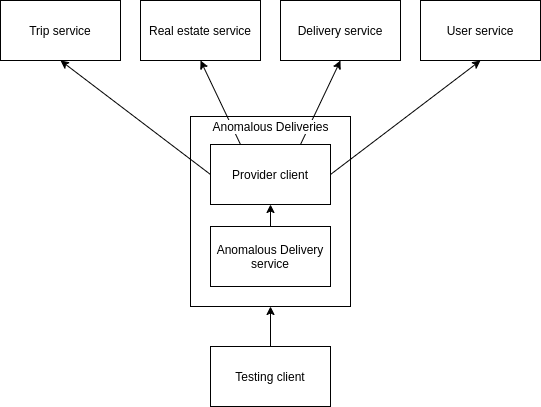
\includegraphics[scale=0.5]{thesis_svava/images/architecture.png}}
    \caption{The architecture for each service.}
    \label{fig:architecture}
\end{figure}

Each service implemented 5-6 methods/endpoints for fetching the data. These methods were based on the existing methods in the four Picnic microservices:
\begin{itemize}
    \item \texttt{getDeliveryById}: Accepts a single string parameter, returns a Delivery.
    \item \texttt{getDeliveryIdsByTripId}: Accepts a single string parameter, returns a list of strings.
    \item \texttt{getDistributionCenterById}: Accepts a single string parameter, returns a DistributionCenter.
    \item \texttt{getUserById}: Accepts a single string parameter, returns a User.
    \item \texttt{getTrips}: Accepts two date-time objects and a string, returns a list of Trips with a matching distributionCenterId which have a start time which falls between the two time instances supplied.
\end{itemize}
In addition, REST, RSocket and gRPC also implemented a sixth method:
\begin{itemize}
    \item \texttt{getTripOverviews}: Same parameters as \texttt{getTrips}, but returns a list of \texttt{TripOverviews}. Each \texttt{TripOverview} has all the same fields as a Trip, as well as a list of \texttt{DeliveryOverviews}. Similarly, each \texttt{DeliveryOverview} has the same fields as a \texttt{Delivery}, as well as a field for the respective User.
\end{itemize}
This method allows the other three services to fetch a collection of trips, the deliveries associated with them and the users associated with the deliveries, in a single request. The same was not needed for GraphQL, since GraphQL allows clients to specify which fields are needed, so \texttt{Deliveries} and \texttt{Users} can be included or omitted without any change in which method is called.

GraphQL and gRPC both offer the option of defining the set of fields in a resource deemed relevant for clients; GraphQL through its schema and gRPC through the proto file. Thus, for all resources the expected size of returned resources should be much smaller than for RSocket and REST. As an example, the \texttt{User} Java class imported from the Picnic ecosystem and returned in full by REST and RSocket contains 24 fields of types ranging from primitive (string), to complex, to sets of either type. In contrast, GraphQL and gRPC each only return 4 fields of a user, the \texttt{userId}, \texttt{firstname}, \texttt{lastname} and \texttt{contactEmail}.

\section{Implementation and deployment}
The services were all developed in Java Spring. That is both the technology of choice within Picnic, as well as convenient since a Spring Boot configuration already existed for each of the four communication methods. Efforts were made to keep the development of each service as homogeneous as possible, to ensure the performance was only affected by the specifics of each communication protocol/style. This included using Reactor for any reactive components, Jackson for serializing JSON (except for gRPC, which uses protocol buffers) and (where possible) using the same Java objects for the same resource (usually the ones defined in the existing microservices of Picnic). GraphQL and REST both use the Spring Webflux framework for HTTP communication and all four services use Netty as the server framework. 

Each service was wrapped in a Docker container and deployed to a Kubernetes cluster, to mimic the setup of a typical service within Picnic. The same configuration was used for each one to make sure no external variables affected their performance. 

\chapter{Experiment design}
In this chapter, the design and implementation of the test cases used as the basis for the experiment will be discussed, as well as the metric used for the performance measurements.

\section{Test cases}
The primary goal of the experiments was to measure the overall time it took to execute a test case, thus providing insight into the latency of the different communication methods and the differences in performance. All the testing code was developed with Node.js and using the core module \texttt{perf\_hooks}, a time measurement was taken right before each test case iteration was set off. Another measurement was taken as soon as all data had arrived from the server, and the difference of these two measurements (in milliseconds) written to a file to register the total time taken to request and receive all the data required by the test case. Any work needed to set up connections before a request was made (as is needed for RSocket and gRPC) was included in the performance measurement to ensure a fair comparison. Furthermore, measures were taken to ensure the network conditions were also fair, by running all tests at the same place, with the same network setup and at around the same time of day.

For each service, five test cases were defined, with the exception of GraphQL which had four (further explained below). These five test cases were designed to test a variety of scenarios representing real-world use cases, with a mix of single and multiple resources and sequential and parallel execution. The five test cases are as follows:
\begin{enumerate}
    \item Single resource: A single request-response for a single resource
    \item Multiple related resources
    \begin{enumerate}
        \item \textit{In one request}: Fetch all resources in one ad-hoc request. The logic for connecting the resources together is on the server side.
        \item \textit{In multiple requests} : Sequentially fetching each resource type in a separate request, connecting the resources together client-side.
    \end{enumerate}
    \item Multiple unrelated resources
    \begin{enumerate}
        \item \textit{Parallel}: Initiate the requests asynchronously and wait until all have returned a response.
        \item \textit{Sequential}: Initiate the requests in sequence and wait until the last one has returned a response.
    \end{enumerate}
\end{enumerate}
As mentioned before, only four of these test cases were performed on GraphQL. Test case 2.B. was excluded for GraphQL. GraphQL's query structure and query resolving functionality is based on the idea that such requests can always be done in one request and thus, artificially fetching the data in multiple requests when no extra effort is needed to do it in one was deemed pointless, as that would not be done in a real world setting.
A similar argument could be made for REST. REST is designed around the principle of fetching a single resource (type) at a time, so creating an ad-hoc endpoint that fetches several at once would go against that principle. However, since developers might be tempted to create such endpoints to circumvent the issue of under-fetching, the decision was made to test the performance of those as well, to see whether these ad-hoc endpoints offer a sufficient performance advantage that could convince developers to stick with HTTP endpoints rather than spend time and money on switching to another protocol (such as GraphQL).
For gRPC and RSocket, no principles have been introduced that dictate which method of fetching multiple related resources should be used. Thus, to ensure a complete comparison, both test cases were applied.

\section{Test implementation}

The five test cases were implemented based on fetching the following resources:
\begin{enumerate}
    \item A single user.
    \item All trips beginning in a certain time period, for a certain distribution center, then all delivery IDs associated with each trip. Next, each delivery associated with these delivery IDs and finally the user associated with each delivery.
    \item A single user, a single distribution center and a list of delivery IDs for a single trip.
\end{enumerate}
For test cases 2.A. and 2.B., the process was as follows:
\begin{itemize}
    \item 2.a: All resources fetched by supplying the initial parameters of the time period and distribution center ID.
    \item 2.b: Trips fetched by supplying the same initial parameters. The trip IDs were extracted from the results, and used to fetch the list of delivery IDs for each trip. Those were then used to fetch each delivery, after which the user IDs were extracted from each to fetch the respective user.
\end{itemize}
For test cases 3.A. and 3.B., the three requests were performed respectively in parallel (firing off each in sequence without waiting for the results of the previous) and in sequence (only firing off a request when all data from the previous has been received).

These five test cases (four in the case of GraphQL) were all performed 100 times each \footnote{The tests were also performed with 1000 iterations with similar results, which indicates that 100 was high enough to give statistically significant results.}, in sequence with a 0.5 s delay between runs to ensure the previous run was not affecting the next one. In total, 19 tests were run and 19 sets of measurements collected, resulting in 5 comparisons that are detailed in graphs in chapter \ref{sec:results}. The results for test case 2 for GraphQL is represented in both the graphs for test case 2a as well as for test case 2b.

RSocket and gRPC both offer the functionality of reusing the connection established for multiple requests. In gRPC, this is the default, unchangeable mechanism and performed under the hood. RSocket offers more control and allows the developer to decide exactly when and how the connection is reused. To ensure a fair and realistic comparison, both protocols were tested with the setup where each iteration used a single connection, no matter how many requests were performed in that iteration. Thus, for the 100 iterations, 100 connections were established. This was done to mimic the behavior of 100 different clients connecting to the server.

\chapter{Results} \label{sec:results}
In this chapter, the results of the experimentation will be presented. For each test case, a box plot is drawn showing the average response times of each of the four services, accompanied by an explanation of the results as well as a small discussion about the possible explanations for the results. The box plots are drawn without outliers \footnote{The boxplots were drawn using R Studio, and to exclude the outliers, the parameter \texttt{outline=FALSE} was supplied. With this option, any point that lies outside the whiskers of the plot, or further from the median than 2.5 times the distance between the median and the relevant quartile, is considered an outlier.} to increase the readability of the graphs, but all data points are included in any other calculation and statistical analysis.

\section{Test case 1}
Figure \ref{fig:stagger_1} shows the results of test case 1, fetching a single delivery. The results are very similar for all four services. GraphQL has a median response time of 121.31 \textit{ms}, gRPC has 127.36 \textit{ms}, REST has 122.77 \textit{ms} and RSocket has 124.00 \textit{ms}. All four required a single request to retrieve the data.

\begin{figure}[ht!]
    \centerline{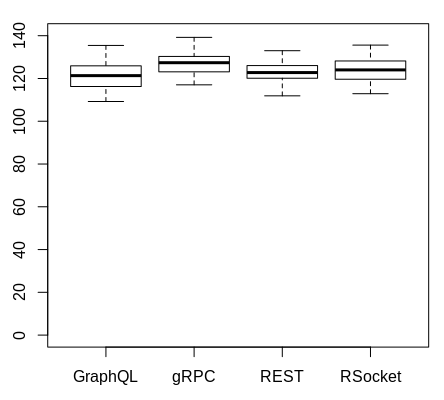
\includegraphics[scale=0.7]{thesis_svava/images/stagger1new.png}}
    \caption{Test case 1: Response times (\textit{ms}) of fetching single delivery.}
    \label{fig:stagger_1}
\end{figure}

\section{Test case 2.A.}
Figure \ref{fig:stagger_2a} shows the results of test case 2.A., fetching a collection of trips, deliveries and users in a single (ad-hoc) request. GraphQL and gRPC show a similar performance with median response times of 182.59 and 179.64 \textit{ms}, respectively. RSocket is slightly slower with 217.69 \textit{ms} response time, and REST comes in last with a median response time of 315.26 \textit{ms}. All four services required a single request to retrieve all data.

While the performances for RSocket, gRPC and GraphQL are similar here, these results show that even if a custom ad-hoc HTTP endpoint is used in an otherwise RESTful service, the performance can still not keep up with the other protocols.

\begin{figure}[ht!]
    \centerline{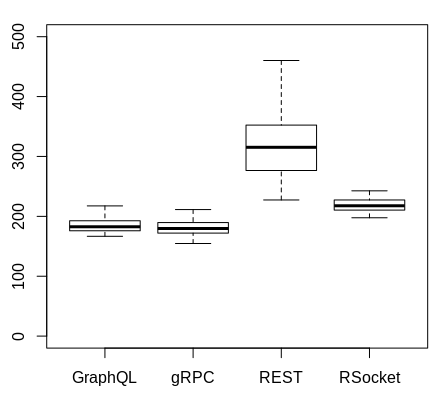
\includegraphics[scale=0.7]{thesis_svava/images/stagger2anew.png}}
    \caption{Test case 2.A.: Response times (\textit{ms}) of fetching trips, deliveries and users in a single request.}
    \label{fig:stagger_2a}
\end{figure}

\section{Test case 2.B.}
Figure \ref{fig:stagger_2b} shows the results of test case 2.B., fetching the same set of objects as 2.A. but in separate requests per resource type for REST, RSocket and gRPC. The result-set for GraphQL here is the same as in Figure \ref{fig:stagger_2a}. GraphQL is now fastest with the median response time of 182.59 \textit{ms}. Next is RSocket, with a 341.59 \textit{ms} response time followed closely by gRPC with 406.99 \textit{ms}. Finally, REST is again the slowest with a median response time of 482.42 \textit{ms}. GraphQL again required only one request, while the other three required in total 30 requests each.

This test case showcases especially well how the GraphQL feature of fetching multiple connected resources in one request improves performance. Furthermore, the performance of gRPC and RSocket is better than for REST, most likely due to the connection reuse feature that both offer.

\begin{figure}[ht!]
    \centerline{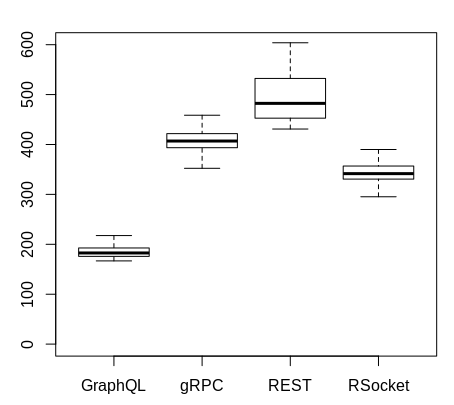
\includegraphics[scale=0.7]{thesis_svava/images/stagger2bnew.png}}
    \caption{Test case 2.B.: Response times (\textit{ms}) of fetching trips, deliveries and users in multiple requests (except GraphQL).}
    \label{fig:stagger_2b}
\end{figure}

\section{Test case 3.A.}
Figure \ref{fig:stagger_3a} shows the results of fetching three different resources in one request each, in parallel. The results are again similar (although not as close as in test case 1) for all four services. GraphQL has a median response time of 130.46 \textit{ms}, gRPC has 142.62 \textit{ms}, REST has 128.65 \textit{ms} and RSocket has 125.26 \textit{ms}.

\begin{figure}[ht!]
    \centerline{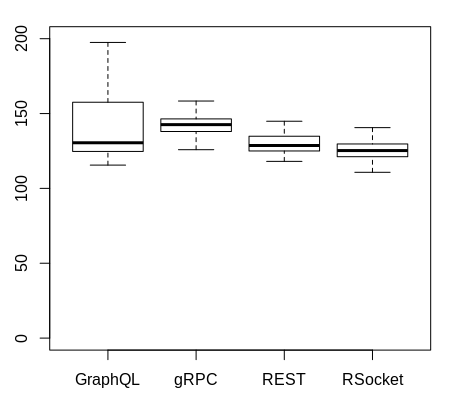
\includegraphics[scale=0.7]{thesis_svava/images/stagger3anew.png}}
    \caption{Test case 3.A.: Response times (\textit{ms}) of fetching a user, a distribution center and delivery IDs in multiple, parallel requests.}
    \label{fig:stagger_3a}
\end{figure}

\section{Test case 3.B.} \label{sec:stagger_3b}
Figure \ref{fig:stagger_3b} shows the results of fetching the same set of objects as 3.A., but in sequence rather than parallel. RSocket now is the fastest with a median response time of 220.19 \textit{ms}. Next is gRPC with a median response time of 294.07 \textit{ms}. Finally, GraphQL and REST have similar results, with median response times of 360.70 and 363.09 \textit{ms}, respectively.

The reason the connection reuse doesn't impact the performance as much in the parallel test case can be explained by the fact that when the three requests are performed in parallel, they are all being handled by the same connection, which could be putting an extra load on that connection. The load thus could be counteracting the benefit provided by not having to re-establish the connection. However, when performed in sequence, the connection only handles one request at a time, so the connection reuse benefit can be enjoyed.

\begin{figure}[ht!]
    \centerline{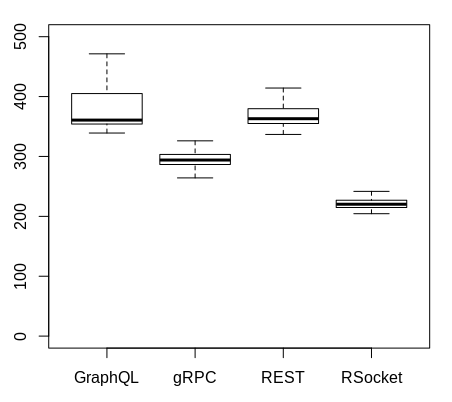
\includegraphics[scale=0.7]{thesis_svava/images/stagger3bnew.png}}
    \caption{Test case 3.B.: Response times (\textit{ms}) of fetching a user, a distribution center and delivery IDs in multiple, sequential requests.}
    \label{fig:stagger_3b}
\end{figure}

The results of these five test cases can be seen in table \ref{tab:results}

\begin{table}
\centering
\label{tab:results}
\begin{tabular}{l|l|l|l|l}
             & GraphQL & gRPC   & REST   & RSocket  \\ 
\hline
Test case 1  & 121.31  & 127.36 & 122.77 & 124.00   \\ 
\hline
Test case 2.A. & 182.59  & 179.64 & 315.26 & 217.69   \\ 
\hline
Test case 2.B. & 182.59  & 406.99 & 482.42 & 341.59   \\ 
\hline
Test case 3.A. & 130.46  & 142.62 & 128.65 & 125.26   \\ 
\hline
Test case 3.B. & 360.70  & 294.07 & 363.09 & 220.19  
\end{tabular}
\caption{Median response time in ms of the five test cases.}
\end{table}

\section{Extra test case - connection reuse}
\begin{figure}
    \centerline{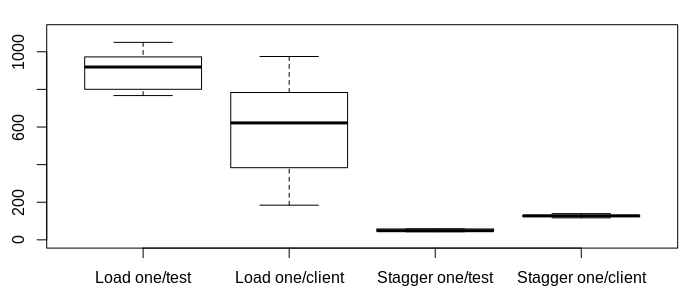
\includegraphics[scale=0.6]{thesis_svava/images/grpcconnections.png}}
    \caption{Response times (\textit{ms}) of gRPC fetching a single delivery.}
    \label{fig:conn_reuse_g}
\end{figure}
\begin{figure}
    \centerline{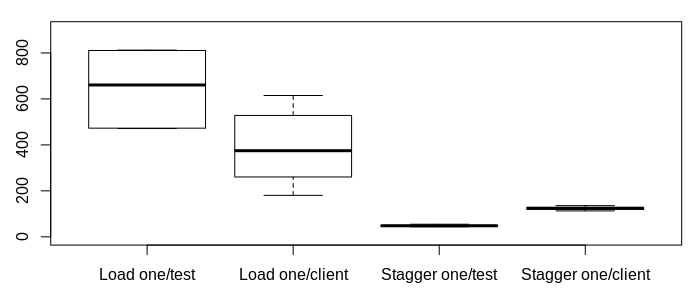
\includegraphics[scale=0.6]{thesis_svava/images/rsocketconnections.png}}
    \caption{Response times (\textit{ms}) of RSocket fetching a single delivery..}
    \label{fig:conn_reuse_r}
\end{figure}
To further illustrate the effect discussed in section \ref{sec:stagger_3b}, two extra tests were performed on RSocket and gRPC: using the same connection for all 100 iterations. Test case 1 was chosen for this. The results obtained previously were compared with a test where all 100 iterations were set off in parallel. The results for each service can be seen in Figures \ref{fig:conn_reuse_r} and \ref{fig:conn_reuse_g}. In both plots, "stagger" refers to the sequential test run with a 0.5 s delay between iterations while "load" refers to the test wherein all iterations are run concurrently.

For both services, we can see that in the staggered mode, the performance is better when using one connection for all 100 iterations since the connection has a chance to "cool down" between requests. However, when running all 100 iterations concurrently, the performance is much better when a new connection is established for each iteration. Here, the performance degradation induced by overloading the single connection far outweighs the benefits of not having to re-establish the connection.

This indicates that for use cases where a single client has to issue a great number of requests to the same server in a short time frame, it may in fact be better to spread the load over multiple connections rather than to reuse the same one.

\chapter{Discussion}
The results of the five test cases have been shown to support the claims of developers of the three communication methods GraphQL, RSocket and gRPC that services can benefit performance-wise from using them over RESTful HTTP APIs. 

In the standard case of submitting a single request for a single resource, the four methods all perform similarly. In the case where a single request is made for multiple connected resources, REST has a significantly worse performance. GraphQL and gRPC likely perform better than REST here due to their schema/protobuf which enables the avoidance of sending fields not needed for the use case at hand. RSocket does not offer this advantage, however its binary encoding is possibly contributing to its better performance than REST. As mentioned in the results section, this test case does show that using ad-hoc endpoints that do not fit with the RESTful architectural constraints can not achieve the same performance benefits as the other technologies, even though that is a common workaround for the problem of under-fetching.

However, in cases where other methods require multiple requests to fetch data where GraphQL can do it in one, GraphQL outperforms the others. In contrast, where all four technologies require the same number of requests, GraphQL does not outperform the others. This indicates that GraphQL's main advantage is in minimizing the amount of requests needed overall. For systems with complex underlying data models (especially ones based on graphs), this indicates that GraphQL is a very good choice. In a system with a simpler data model and simpler use cases (e.g. where a majority of use cases only depend on a single data resource), using GraphQL would not offer a major performance advantage.

In the cases where all four methods require multiple requests performed in sequence, RSocket and gRPC both benefit greatly from multiplexing by sending all requests over the same connection. Avoiding the overhead incurred by constantly needing to re-establish the connection thus offers a great advantage. For parallel requests however, this benefit could be counteracted by the overloading incurred by sending too many requests over the same connection. Further tests might need to be done to investigate at which point this trade-off switches, to provide guidelines to developers for when to spread the requests over multiple connections, and when using the same connection is sufficient. However, since gRPC does not allow for this in most implementations, in this aspect RSocket has the upper hand.

There are a few limitations with these experiments. Firstly, this thesis did not put any explicit focus on the performance of the data serialization (JSON vs Protocol Buffers). Some studies have been done on this topic, with Popić et al. showing that the size of messages can be minimized by 83\% by using protocol buffers rather than JSON \cite{popic2016performance}. In addition, Wibowo showed that the time taken to serialize messages went from around 10.5 \(\mu s\) with JSON to around 6.5 \(\mu s\) \cite{wibowo2011evaluation}. Given that gRPC was the only one out of the four that did not use Jackson for JSON serialization, it is possible that this gave gRPC an unfair advantage over the others. However, since most documentation and tutorials assume the usage of protocol buffers, the choice was made to use it as:
\begin{enumerate}
    \item There are few resources available that explain how to use other serialization methods.
    \item In practice, protocol buffers would most likely be used due to their status as the default serialization method.
\end{enumerate}
Thus, to emulate a real-world scenario, it was considered more prudent to use gRPC with protocol buffers. 

Next, the selection of the 0.5 second interval between requests in the experiments was not properly supported with arguments. Other theses with similar focus opted for either a 1 second interval \cite{johansson2017efficient} or a 0.5 second interval \cite{cederlund2016performance}. However, it would have been better to perform additional tests to see whether the 0.5 second interval was long enough to allow the services to cool down between requests. If any of the services require a longer time to cool down than the others, their performance would have been affected. This was not taken into consideration and could have changed the final conclusion. 

Finally, the author originally intended to also do experiments to see whether the four services behaved differently under load, which could provide insight into which of the four is best suited for larger systems with greater performance in high-traffic periods. However, due to time constraints this was not possible.

\chapter{Conclusions}
Among the four communication technologies discussed in this thesis, GraphQL, gRPC and RSocket all seem to be a better fit for microservice architecture than REST. For inter-service communication, REST lacks many of the features that give the other three increased performance, such as multiplexing, header compression, more efficient encoding or flexible client-defined queries. The experimental results showcase this, attested by the fact that REST never had the best performance out of the four in any test case. REST suffers from the fact that it is a style developed long before microservice architecture was popularized. It is designed for HTTP communications focusing on hypermedia intended for display in browsers. Within the microservices world, REST is most appropriate for client-facing APIs but even then, the issues of under- and over-fetching can cause worse performance as well as lead developers to rely on ill-designed workarounds that break the constraints of REST. However, since REST has been so popular since its inception, most web and back-end developers are very familiar with it. For simpler systems with simpler use cases, REST still serves its purpose.

For similar reasons, GraphQL is also better suited for client-facing APIs than for inter-service communications. It has several advantages over REST, mainly due to its strongly typed schema and client-defined queries. A single GraphQL request can have the same performance as a single REST request but the ability to easily query for multiple resources with a single request without having to define a specific method/endpoint for it gives GraphQL a considerable edge not just on REST, but also on gRPC and RSocket as was shown in figure \ref{fig:stagger_2b}. For microservices systems with complex underlying data models (especially ones structured as graphs) and/or serving multiple clients with different needs, GraphQL is a good choice.

In contrast, gRPC and RSocket are better suited for inter-service communications than both REST and GraphQL, each being designed explicitly for microservices communications. The two show very similar performance results, with the same result in the first test case, gRPC being slightly faster in the second and RSocket slightly faster in the other three. For both, the impact of a high number of simultaneous requests over a single connection decreased the performance, indicating that spreading the requests over multiple connections could improve the overall performance. However, RSocket allows much more control over this than gRPC, with implementations of gRPC implicitly reusing the connection within the same process even when the developer explicitly attempts to open a separate one. Both technologies offer multiple interaction models, multiplexing and reduced bandwidth either through header compression or binary encoding. RSocket however has an advantage over gRPC in not adhering to the client-server model, allowing communicating services to act more like peers. Finally, the default usage of protocol buffers in gRPC can put it either at an advantage or disadvantage, depending on the requirements of the system at hand. The strong typing offered can be safer and provides better understanding between different teams of the interface behavior and the code generation can save time in development, however it limits flexibility and freedom over what can be sent over the network. gRPC is also tied to HTTP/2, while RSocket can use any byte stream protocol, even different ones in the same service.

Ultimately, the choice of a technology not only depends on the architecture chosen for a system, but also the experience and preference of the developers, the specifics of the use case, complexity of the system and data model, and the performance requirements. It would be near impossible to design one protocol or framework which is perfect for microservices in every way. However, it should always be possible, through careful analysis, to find the approach that works the best for the case at hand. For Picnic's use case, the author's recommendation would be GraphQL for client-facing APIs due to its better performance and flexible querying, and RSocket for inter-service communications due to the freedom and control it provides.

          
%\include{9_appendix/appendix}
      
            
% --------------------------------------------------------------
%:                  BACK MATTER: appendices, refs,..
% --------------------------------------------------------------

% the back matter: appendix and references close the thesis


%: ----------------------- bibliography ------------------------

% The section below defines how references are listed and formatted
% The default below is 2 columns, small font, complete author names.
% Entries are also linked back to the page number in the text and to external URL if provided in the BibTex file.

% PhDbiblio-url2 = names small caps, title bold & hyperlinked, link to page 
%\begin{multicols}{2} % \begin{multicols}{ # columns}[ header text][ space]
%\begin{tiny} % tiny(5) < scriptsize(7) < footnotesize(8) < small (9)

\bibliographystyle{Latex/Classes/PhDbiblio-url2} % Title is link if provided
\renewcommand{\bibname}{References} % changes the header; default: Bibliography

\bibliography{11_references/references} % adjust this to fit your BibTex file

%\end{tiny}
%\end{multicols}



% --------------------------------------------------------------
% Various bibliography styles exit. Replace above style as desired.

% in-text refs: (1) (1; 2)
% ref list: alphabetical; author(s) in small caps; initials last name; page(s)
%\bibliographystyle{Latex/Classes/PhDbiblio-case} % title forced lower case
%\bibliographystyle{Latex/Classes/PhDbiblio-bold} % title as in bibtex but bold
%\bibliographystyle{Latex/Classes/PhDbiblio-url} % bold + www link if provided

%\bibliographystyle{Latex/Classes/jmb} % calls style file jmb.bst
% in-text refs: author (year) without brackets
% ref list: alphabetical; author(s) in normal font; last name, initials; page(s)

%\bibliographystyle{plainnat} % calls style file plainnat.bst
% in-text refs: author (year) without brackets
% (this works with package natbib)


% --------------------------------------------------------------

% according to Dresden med fac summary has to be at the end
%
% Thesis Abstract -----------------------------------------------------


%\begin{abstractslong}    %uncommenting this line, gives a different abstract heading
\begin{abstracts}        %this creates the heading for the abstract page

Microservices have gained interest in the last years, often as an alternative to monolithic applications. Microservice architecture revolves around independent services communicating over network interfaces. For them to be a viable alternative to an application in which all components can communicate locally (as is the case in monoliths), it is important that the network communication is efficient and has good performance. REST (REpresentational State Transfer) over HTTP is the most commonly used method of communication in microservice systems, but in recent years GraphQL, gRPC and RSocket have all been introduced as alternatives to REST. This thesis aims to evaluate the suitability of these four technologies for microservices, both through a comparative analysis of their architectures and through performance experiments based on a case study for Picnic Technologies. The results of this evaluation indicate that RSocket and gRPC are well suited for inter-service communication, both showing good performance in multiple cases. Their differences lie mainly in their architecture, with gRPC being an RPC client-server framework built over HTTP/2 while RSocket is a binary protocol with symmetric interaction models intended for byte stream transport such as TCP. On the other hand, GraphQL and REST are both better suited for client-facing APIs. Performance-wise, GraphQL does especially well for complex use cases, while REST performs the worst overall out of the four. GraphQL's schema, graph-based approach and client defined queries make it a good choice for more complex microservice architectures.
\end{abstracts}
%\end{abstractlongs}


% ---------------------------------------------------------------------- 


%: Declaration of originality
%\include{8_backmatter/declaration}



\end{document}
